\documentclass[titlepage]{article}
\usepackage{graphicx}
\usepackage{fancyhdr}
\usepackage{hyperref}
\usepackage{tabularx}
\usepackage{multicol}

\title{FC Package}
\author{
	Andrew Borba\\ \emph{Prototyper}	\and
	 Elisabeth Brooks\\ \emph{Project Manager}	\and
	 Jorge Go\\ \emph{Feasability Analyst}	\and
	 Katherine Hu\\ \emph{Lifecycle Planner}	\and
	 Nakul Joshi\\ \emph{Software Architect}	\and
	 Ian Malave\\ \emph{Requirements Engineer}	\and
	 Rishi Mukhopadyay\\ \emph{Operational Concept Engineer}
}
\date{November 1\textsuperscript{st}, 2013}

\begin{document}
\pagestyle{fancy}
\lhead{FC Package}
\chead{}
\rhead{Version 2.1}
\lfoot{}
\cfoot{\thepage}
\rfoot{}

\maketitle
\tableofcontents
\newpage
\section{Version History}
\begin{table}[h]
	\centering
	\begin{tabularx}{\textwidth}{lllXX}
		\hline
		Date		& Author	& Version	& Changes Made											& Rationale                    \\ \hline
		08/20/2013	& SK		& 1.0		& Original for CS 477; Tailored from ICSM REQ Template	& To fit CS 477 Course Content \\ 
		09/14/2013	& Team 1	& 1.1 		& First version											& Project Requirements			\\
		10/15/2013	& Team 1	& 2.0 		& Shifted marketing focus from LA Metro to TAP			& Reassesment of stakeholder values\\
		11/01/2013	& Team 1	& 2.1		& Fixed various design flaws											& Incorporated feedback from ARB review board
	\end{tabularx}
\end{table}
\newpage

\section{Team Members}
\subsection{Schedule}
Until we get the schedule for next semester with more specific dates, we are only able to identify some key phases and tasks that we will need to complete, but we cannot attach them to dates. Additionally, as we work more on development, this schedule may change as we face challenges, or finish tasks quicker than we estimated. Our current schedule overview and plan is as follows:\begin{description}
\item[January –- February]Work with Teams\begin{itemize}
	\item Rebaseline prototype, prioritize requirements
	\item Plan for CS477b specifics, including transition strategy
	\item Participate in ARB review
\end{itemize}
\item[February –- May]Scheduled Weekly Meetings to:\begin{itemize}
	\item Discuss status and plans
	\item Provide access to key transition people for strategy and readiness discussions 
\end{itemize}
\item[March 3--7]Iteration Assessment Reviews
\item[March 26]Core Capability Drivethrough
\item[April 14--18]Project Transition Readiness ARB Reviews
\item[April 21]Installation and Transition\begin{itemize}
	\item Install Product
	\item Execute Transition Plan
\end{itemize}
\item[April 28]Operational Commitment Review for Initial Operational Capability
\item[May 5]Client Evaluations
\end{description}

\clearpage

\subsection{Project}
We have created a project using Microsoft Project to track tasks, phases, and progress. These will be drastically updated as we are provided a more specific schedule of requirements, however sample charts can be seen below.
\begin{figure}[!htbp]
\centering
\includegraphics[scale=0.7]{images/completeness.png}
\end{figure}
\begin{figure}[!htbp]
\centering
\includegraphics[scale=0.7]{images/graph.png}
\end{figure}

\clearpage

\subsection{Phases and Milestones}
Phases planned in the second semester include the end of the Foundations Phase, the Development Phase, which has two parts, construction and transition, and the Operations Phase. 
Milestones include the RDCR (Rebaselined Development Commitment Review), CCD (Core Capability Drivethrough), TRR (Transition Readiness Review) and OCR (Operational Commitment Review). 
Our tentative schedule of necessary phases and milestones is below:

\begin{figure}[!htbp]
\centering
\includegraphics[scale=0.5]{images/table1.png}
\end{figure}
\begin{figure}[!htbp]
\centering
\includegraphics[scale=0.5]{images/table2.png}
\end{figure}
\begin{figure}[!htbp]
\centering
\includegraphics[scale=0.5]{images/table3.png}
\end{figure}

\subsection{Team}
For our team structure and roles, we will have each member coding, testing, and reviewing the work of someone else on the team. We plan to have peer coding, where two people code together. While each member will be have multiple roles and responsibilities, we have broken the team up into front-end and back-end, testers and trainers, and then each member will be an implementer. As the semester of 477b progresses, we may update these roles as we feel necessary, depending on how we progress. 
The following charts lists the team structure and each team member, their positions for 477a/b, and their tentative roles and responsibilities. As we begin work, these may change due to what the team needs.

\begin{figure}[!htbp]
\centering
\includegraphics[width=0.7\textwidth]{images/implementation.pdf}
\caption{Team Structure: Implementation}
\end{figure}

\begin{figure}[!htbp]
\centering
\includegraphics[width=0.7\textwidth]{images/testingtraining.pdf}
\caption{Team Roles: Testing and Training}
\end{figure}

\clearpage

% Please remember to add \use{multirow} to your document preamble in order to suppor multirow cells
% Booktabs require to add \usepackage{booktabs} to your document preamble
\begin{table}[h]
\begin{tabularx}{\textwidth}{@{}llX@{}}
\toprule
Team Member                                                 & Role                          & Responsibility                                               \\ \midrule
Elisabeth Brooks                                            & Project Manager               & Create and manage schedules                                  \\
                                                            &                               & Maintain project management tool (Asana)                     \\
                                                            &                               & Hold team members accountable                                \\
Ian Malave                                                  & Requirements Engineer         & Develop front-end and prototype                              \\
                                                            & Front End Developer           & Update requirements to match prototype                       \\
Andrew Borba                                                & Prototyper                    & Create application prototypes                                \\
                                                            & Front End Developer           & Develop the front-end                                        \\
Katherine Hu                                                & Life Cycle Planner            & Validate application design                                  \\
                                                            & Front End Developer           & Ensure user-friendliness and legibility                      \\
Nakul Joshi                                                 & Systems Architect             & System \& security design on high-level back-end development \\
                                                            & Back End Developer            & Manage LaTeX documentation                                   \\
Jorge Go                                                    & Feasibility Analyst           & Identify and analyze risks                                   \\
                                                            & Back End Developer            & Plan risk mitigation strategies                              \\
                                                            &                               & Run business case and cost-benefit analysis                  \\
Rishi & Operational Concept & Implement back-end                                           \\
Mukhopadyay                                                        & Engineer           & Plan database structure              \\
& Back End Developer &                       

\\ \bottomrule
\end{tabularx}
\end{table}
\newpage

\section{Client Interaction Report}
\section{Client Interaction Report}
\subsection{Current Infrastructure}
The LA Metro Bus currently has a few options when it comes to purchasing redeeming tickets. Riders can either purchase single-ride fares on the bus or pay using pre-purchased tokens. For both these options the rider receives a paper ticket as a proof of purchase. Another option is for metro users to purchase a TAP card from many locations across Los Angeles, and be refilled from any TAP vending machine. To use these TAP cards, users simply tap their card as they enter the bus and the appropriate fare is deduced. The initial cost for the TAP card is \$1 and can store values for up to three years. 

There is currently no competitor for the TAP concept since it is produced and run by a government agency. The current options are either using a TAP card or pay as you go. Our product would save resources, time, and create a more user friendly interface and payment options.

\subsection{Current Artifacts}
\begin{table}[h]
    \begin{tabularx}{\textwidth}{lXlr}\hline
    Artifact              & Description                                              & Status & Planned Delivery Date          \\
    \hline
    Requirements          & Written list of requirements for the app                 & Requested                   & 09/07/2013                              \\
    Architecture          & Structure of the app                                     & Requested                   & 11/01/2013                              \\
    Life-cycle plan       &  Documentation of release cycle and list of new features & Requested                   & 12/01/2013                             \\
    Feasibility evidence  & Documentation of feasibility of the application and use  & Requested                   & 12/01/2013                              \\
    \hline
    \end{tabularx}
\end{table}
\newpage
\subsection{Current Business Workflow}
\begin{figure}[h]
\centering
\includegraphics[scale=.5]{CIR/uml.pdf}
\end{figure}
\newpage

\section{Operational Concept Description}


\subsection{Shared Vision}

	\subsubsection{System Overview}\begin{multicols}{2}
				\paragraph{Key Partners}\begin{enumerate}
			\item TAP
		\end{enumerate}
		
		\paragraph{Key Activities}\begin{enumerate}
			\item Software Design and Development
			\item Integration with Metro  infrastructure
			\item Marketing of application
		\end{enumerate}
		
		\paragraph{Key Resources}\begin{enumerate}
			\item Development Team
			\item PhoneGap API
			\item NFC technology
			\item QR technology
		\end{enumerate}
		
		\paragraph{Value Proposition}\begin{enumerate}
			\item Convenience for customers to purchase and use metro tickets
			\item Ticket elimination reducing cost and environmental impact
			\item Technological advancement of public transportation system. 
 		\end{enumerate}
 		
 		\paragraph{Customer Relation}\begin{enumerate}
 			\item LA Metro
 			\item Apple Appstore
 			\item Android Store
 			\item Windows Phone Marketplace
 		\end{enumerate}

 		\paragraph{Channels}\begin{enumerate}
 			\item Application stores
 			\item LA Metro website
 			\item Posters and billboards at stations. 
 		\end{enumerate}
 		
 		\paragraph{Customer Segments}\begin{enumerate}
 			\item Transportation Companies
 		\end{enumerate}
 		
 		\paragraph{Cost Structure}\begin{enumerate}
 			\item Development Team
 			\item Back-end System Administrator
 		\end{enumerate}
 		
 		\paragraph{Revenue Streams}\begin{enumerate}
 			\item Flat fee for project implementation
 			\item Recurring fee per ticket sale through application
 		\end{enumerate}
	\end{multicols}
 	\newpage

 	\subsubsection{System Boundary and Environment}
 	\begin{figure}[h]
 		\centering
 		\includegraphics[scale=0.5]{OCD/boundary2.pdf}
 	\end{figure}
 	\newpage
 		
\subsection{System Transformation}
	\subsubsection{System Objectives, Constraints, and Priorities}
		

% Booktabs require to add \usepackage{booktabs} to your document preamble
\begin{table}[h]
\begin{tabularx}{\textwidth}{Xl}
\toprule
Capability Goals                                                                             & Priority Level                                                           \\ \midrule
\textbf{OC-1} Cross-platform Compatible:                                                              & Must have                                                                \\
\multicolumn{2}{X}{The application is compatible with iOS, Android and Windows Phone}                                                                                   \\
\textbf{OC-2} Account Creation:                                                                       & Must have                                                                \\
\multicolumn{2}{X}{The application is able to create new rider accounts, update information, and log in users using existing information.}                              \\
\textbf{OC-3} Usage:                                                                                  & Must have                                                                \\
\multicolumn{2}{X}{The application allows metro riders to board trains via NFC or QR code technology.}                                                                  \\
\textbf{OC-4} Payments:                                                                               & Must have                                                                \\
\multicolumn{2}{X}{The application allows metro riders to pay for tickets using a secure payment gateway and will allow metro riders to store credit card information.} \\
\textbf{OC-5} Schedules:                                                                              & Should have                                                              \\
\multicolumn{2}{X}{The application allows metro riders to view train schedules.}                                                                                        \\
\textbf{OC-6} Map:                                                                                    & Should Have                                                              \\
\multicolumn{2}{X}{The application allows metro riders to view a static map of metro stations.}                                                                         \\
\textbf{OC-7} Updates:                                                                                & Should Have                                                              \\
\multicolumn{2}{X}{The application allows metro riders to receive updates about train station information and irregular service interruptions.}                         \\
\textbf{OC-8} Pricing:                                                                                & Should Have                                                              \\
\multicolumn{2}{X}{The administration application will allow metro administrators to change ticket pricing.}                                                            \\
\textbf{OC-9} Ticket Types:                                                                           & Could Have                                                               \\
\multicolumn{2}{X}{The application will support linking of additional tap accounts for the purpose of allowing dependants to be charged with one QR scan.}              \\
\textbf{OC-10} Ticket Display:                                                                        & Should Have                                                              \\
\multicolumn{2}{X}{The application will use GPS services to automatically display tickets for the closest station.}           \\
\bottomrule                                         
\end{tabularx}
\end{table}

% Booktabs require to add \usepackage{booktabs} to your document preamble
\begin{table}[h]
\centering
\begin{tabular}{@{}ll@{}}
\toprule
Level of Service Goals     & Priority Level \\ \midrule
Reliability of application & Must have      \\
Usability                  & Must have      \\
Security                   & Must have      \\
Performance of system      & Should have    \\
Inter-operability          & Should have    \\
Maintainability            & Should have   \\
\bottomrule
\end{tabular}
\end{table}


\paragraph{Organizational Goals}\begin{description}
	\item[OG-1] Increase convenience for ticket buyers.
	\item[OG-2] Decrease cost for LA Metro and ticket buyers. 
	\item[OG-3] Increase efficiency of public transit system by advancing technologically.
\end{description}

\paragraph{Constraints}\begin{description}
	\item[CO-1] Align with Current Infrastructure: The new application must complement the existing tap card system, and be implemented with minimal changes to existing infrastructure. 
	\item[CO-2] Cross Platform Compatibility: The new application must be compatible with major smartphone operating systems(iOS, Android and Windows)
	\item[CO-3] Phone Hardware: The application must be compatible with the existing hardware in major smartphones.

\end{description}
	\newpage
	
	\subsubsection{Proposed Operational Concept}
		The application will allow metro riders to use their mobile devices to purchase tickets and board trains eliminating the need for physical TAP cards. The new system will act as a complement to the TAP card system; allowing riders to use existing metro facilities if they wish.
		
		For those smartphones enabled with NFC, the rider will be able to “tap” their phones instead of their tap cards. For those smartphones not enable with NFC, QR readers will be installed at stations that have turnstiles. For stations that do not have turnstiles, Metro agents will be given a QR reader to verify tickets on the train.

	\subsubsection{Proposed Element Relationship}
		\begin{figure}[h]
			\centering
				\includegraphics[scale=0.45]{OCD/er2.pdf}
		\end{figure}			
	\newpage
	\subsubsection{Proposed Workflow}
		\begin{figure}[h]
			\centering
			\includegraphics[scale=.355]{OCD/uml.pdf}
		\end{figure}
\newpage

\section{Requirements}
\subsection{Capability Requirements}

	\subsubsection{Platform}\begin{enumerate}
		\item The application shall be compatible with the iOS mobile platform.
		\item The application shall be compatible with the Android mobile platform.
	\end{enumerate}
	
	\subsubsection{User Accounts}\begin{enumerate}
		\item If it is a user’s first-time opening the application, the application shall prompt the user to enter an email address, password, credit card information, and to create or link to a TAP account.
		\begin{enumerate}
			\item If the account is created successfully, the application shall send a confirmation to the user’s stored email address.
			\item If the account creation is not successful, the application shall display an error message that prompts the user to reenter their information and will not be logged in.
		\end{enumerate}
		\item If a returning user opens the application, it shall prompt the user to enter their log-in information.
			\begin{enumerate}
				\item If the log-in attempt fails, the application will display an error message that prompts the user to reenter their log-in information.
				\item If the log-in attempt succeeds, the user will be shown a transit management screen.
			\end{enumerate}
		\item The user shall be able to allow the application to automatically sign them in.
		\item The user shall be able to sign out of their account.
	\end{enumerate}
	
	\subsubsection{Usage}\begin{enumerate}
		\item If the application loses connectivity, the application shall display an error message.
		\item The application shall retrieve the user’s location at intervals of 120 $\pm$ 10 seconds.
		\item The application shall allow the user to manually refresh their location.
		\item Upon updating the user’s location, the application shall update information for nearby Metro transportation.
		\item The user shall be able to select which bus or train line is displayed first when the user is nearby a particular Metro station.
		\item The application shall allow the user to change their email address.
		\item The application shall allow the user to change their password.
		\item The application shall allow the user to delete their account.
		\item The user shall be able to link up to 5 dependents (name \& birthdate) to their account.
		\item The user shall be able to link up to 5 dependents TAP accounts to their account.
	\end{enumerate}
	
	\subsubsection{Payments}\begin{enumerate}
		\item The application shall allow users to purchase non-exclusive TAP passes.
		\item If the user selects to purchase a ticket, the application shall check to see if the user has an applicable TAP pass.
			\begin{enumerate}
				\item If the user has an applicable TAP pass, the application shall generate the selected virtual ticket.
				\item If the user does not have an applicable TAP pass, the application shall confirm with the user it will charge the stored credit card.
				\item If the card does not process, an error message shall be displayed and the order shall not be accepted. 
				\item If the transaction succeeds, the application shall create a virtual ticket. 
			\end{enumerate}
		\item If the user has more than one TAP unused pass, the application shall prompt the user to select which to use first.
		\item The user shall be able to select up to 2 dependents’ accounts to be attached to a virtual ticket.
			\begin{enumerate}
				\item If the dependent is over 5 years old, the application shall calculate the additional ticket fare.
			\end{enumerate}
		\item If the user selects to use their ticket, the application shall signal the gate up to a maximum of 3 attempts at 10 $\pm$ 5 second intervals to accept.
			\begin{enumerate}
				\item If the application is unsuccessful on the 3rd attempt, the application shall display an error message.
				\item Otherwise, the gate is unlocked, permitting the user to pass through.
			\end{enumerate}
		\item The application shall store unused virtual tickets for at least 1 year. 
		\item The application shall store used virtual tickets for at least 30 days.
		\item The application shall allow the user to change their credit card information.
		\item The user shall be able to set up the application to generate a default ticket that auto-charges their stored credit card when used.
		\item The application shall support remote adjustment of ticket prices (e.g., senior discount) by TAP id through a web interface.
		\item If the user has an active TAP pass, the application shall display how much time is remaining on the pass.
	\end{enumerate}		
\newpage	
\subsection{Level of Service Requirements}

\begin{table}[h]
    \begin{tabularx}{\textwidth}{Xrr}
    \hline
    LOS Requirements                                                                                          									& Desired Level & Accepted Level \\ \hline
    LOS-1: Concurrent Users														& $150000$		& $75000$           \\
    LOS-2: Start-up and user location time 										& 7 s  			& 15 s           \\
    LOS-3: Ticket Purchase Transaction Time										& 5 s 			& 20 s            \\
    LOS-4: Update Account Information Time										& 10 s 			& 30 s            \\
    LOS-5: Tickets stored per User												& 1500 			& 500            \\
    LOS-6: \% first-time users able to purchase ticket without outside help		& 80  			& 75             \\
    LOS-7: \% first-time users able to use ticket without outside help			& 85 			& 80             \\
    LOS-8: \% users that ride metro at least once per week that would rate 
    ease of use at 3 out of 5 or higher											& 90  			& 80             \\
    LOS-9: Average Time for User to Create an Account							& 45 s			& 60 s            \\
    LOS-10: Failed Ticket Purchases per 1000 									& 0.25  		& 1              \\
    LOS-11: Failed Ticket Uses per 1000  										& 0.25  		& 1              \\
    LOS-12: Hours per day that app shall purchase tickets 						& 20  			& 19.5             \\
    LOS-13: Hours per day that app shall allow use of tickets   				& 20 			& 19.5             \\
    LOS-14: \# iOS generations app shall support 								& 3  			& 2              \\
    LOS-15: \# Android generations app shall support   							& 3  			& 2              \\
    LOS-16: \# versions of app that Metro system shall support  				& 3    			& 2              \\
    \hline
    \end{tabularx}
\end{table}
\newpage

\section{Risk Lists}
\newcommand{\risk}[5]{
	\rule{\textwidth}{.1pt}
	\textbf{ Risk\# #1}(Last week: #2)\\
	\textbf{Weeks Active} #3
	\paragraph{Risk Description} #4
	\paragraph{Mitigation Action Items} #5\\
}



\subsection{Technical Risks}

\risk{1}{1}{7}{
An unsecure platform might be exploited or easily manipulated (e.g. people finding loopholes to avoid fees), which can result in the LA Metro losing profits.
}{
Our group’s architect will develop a cryptosystem for our application that will be tested until it meets the client’s requirements and security standards.
}
\risk{3}{3}{7}{
A technical malfunction of our platform might cause boarding delays for passengers and cause inefficiencies in LA Metro operations.
}{
A back-up system will be designed in a later stage of the project. Also, we will advise passengers who are particularly sensitive to delays to have a back-up physical tap card.
}
\risk{4}{4}{7}{
Not enough end users (passengers) might not have phones on iOS and Android systems that are compatible with our app.
}{
A feasibility study will be conducted to verify iOS/Android penetration rates within the LA Metro passenger base, and if needed, we can tailor our platform to target only a certain segment of the customer base that has access to the required technology.
}
\risk{8}{8}{7}{
We will be using PhoneGap to implement the mobile application with standard web technologies like HTML/CSS/Javascript which makes the application subject to device-specific mobile browser display discrepencies.
}{
Test on a wide variety of devices within iOS/Android space (different iPhone versions and various Android phones) to ensure the application is rendered properly on all screen sizes and OS versions.
}

\subsection{Requirement Risks}
\risk{2}{2}{7}{
TAP might not be willing to implement our system or work with our group to test our platform on their systems/hardware.
}{
Our project manager is currently in talks with TAP, but we could also do a proof of concept using similar hardware/systems or mock interfaces.
}
\risk{6}{6}{7}{
After the platform has been implemented and integrated, the TAP requirements might change, or the technologies being used in relevant processes might change.
}{
If we are under a contract/agreement, the team will develop updates/patches that will adapt to new requirements. Otherwise, we will provide a copy of our comprehensive documentation for the software so that necessary changes can be handled in-house.
}
\risk{5}{5}{7}{
To get the application fully working and integrated into TAP/LA Metro infrastructure, there will be a large set of evolving requirements. Two semesters might not be enough time to complete the project, especially if there are unexpected risks (e.g. another developer completes the same project before we do, bureaucratic risks, etc.)
}{
We will develop a running list of unexpected risks as they come up and develop strategies to approach them. For example, we would explicitly ask TAP for their timeline and ask for an exclusive partnership.
}

\subsection{Human Resources Risks}

\risk{7}{7}{7}{
Due to rapid formation of teams without proper analysis of required skill sets needed for this project we may lack the technical skills to complete this project in a professionally acceptable manner.
}{
Identify team member skills and project requirements so we can individually prepare ourselves for technologies that we will be implementing next semester.
}
\risk{9}{9}{7}{
The statically defined list of team roles may not fit our specific project requirements.
}{
Dynamically reassign team roles as the project and its requirements mature.  Also the team shall be aware that responsibilities will be very flexible and we may need to step outside the scope of our assigned position
}
\risk{10}{10}{7}{
The amount of cooperation needed between our team and TAP may be more than expected which could make this project unfeasible for them.}
{
Come up with a plan focused around the idea that TAP should have to do as little as possible.  Extensive testing should be done internally before our software can be ready for beta testing with TAP.  The goal should be to get it right the first time.
}
\rule{\textwidth}{.1pt}
%\begin{landscape}
%\begin{table}[h]
\begin{center}
\begin{tabularx}{\textwidth}{cccXXc}

1 & N/A & Security & An unsecure platform might be exploited or easily manipulated (e.g. people finding loopholes to avoid fees), which can result in the LA Metro losing profits. & Our group�s architect will develop a cryptosystem for our application that will be tested until it meets the client�s requirements and security standards. & 1 \\ 
2 & N/A & Partnership & The LA Metro might not be willing to implement our system or work with our group to test our platform on their systems/hardware. & Our project manager is currently in talks with the LA Metro authorities, but we could also potentially do a proof of concept using similar hardware/systems. & 1 \\ 
3 & N/A & Technology & A technical malfunction of our platform might cause boarding delays for passengers and cause inefficiencies in LA Metro operations. & A back-up system will be designed in a later stage of the project. Also, we will advise passengers who are particularly sensitive to delays to have a back-up physical tap card. & 1 \\ 
4 & N/A & Technology & End users (passengers) might not have smartphones that have the technical capabilities to support our platform. & A feasibility study will be conducted to verify compatible phone penetration rates, and if needed, we can tailor our platform to target only a certain segment of the customer base that has access to the required technology. & 1 \\ 
5 & N/A & Estimation & To get the application fully working and integrated into the LA Metro system, there will be a large set of evolving requirements. Two semesters might not be enough time to complete the project, especially if there are unexpected risks (e.g. another developer completes the same project before we do, bureaucratic risks, etc.) & We will develop a running list of unexpected risks as they come up and develop strategies to approach them. For example, we would explicitly ask LA Metro for their timeline and ask for an exclusive partnership. & 1 \\ 
6 & N/A & Requirements & After the platform has been implemented and integrated, the LA Metro requirements might change, or the technologies being used in relevant processes might change. & If we are under a contract/agreement, the team will develop updates/patches that will adapt to new requirements. Otherwise, we will give the LA Metro a copy of our comprehensive documentation for the software so that necessary changes can be handled in-house. & 1 \\ 
7 & N/A & People & Due to rapid formation of teams without proper analysis of required skill sets needed for this project we may lack the technical skills to complete this project in a professionally acceptable manner.
 & Identify team member skills and project requirements so we can individually prepare ourselves for technologies that we will be implementing next semester. & 1 \\ 
8 & N/A & Tools & We will be using PhoneGap to implement the mobile application with standard web technologies like HTML/CSS/Javascript which makes the application subject to device-specific mobile browser display discrepencies. & Test on a wide variety of devices (different iPhone versions and various Android phones) to ensure the application is rendered properly on all screen sizes and OS versions. & 1 \\ 
9 & N/A & Organizational & The statically defined list of team roles may not fit our specific project requirements. & Dynamically reassign team roles as the project and its requirements mature.  Also the team shall be aware that responsibilities will be very flexible and we may need to step outside the scope of our assigned position & 1 \\ 
10 & N/A & Estimation & The amount of cooperation needed between our team and LA Metro may be more than expected which could make this project unfeasible for them. & Come up with a plan focused around the idea that LA Metro should have to do as little as possible.  Extensive testing should be done internally before our software can be ready for LA Metro.  The goal should be to get it right the first time. & 1 \\ 
\end{tabularx}
\end{center}
\end{table}

%\end{landscape}

		
\end{document}